\section{The State of Physical Access Control Authentication}
\label{sec:state-of-physical-access-control-authentication}



\subsection{An Overview of Physical Access Control}
\label{subsec:overview-of-physical-access-control}

The purpose of a \ac{pacs} is to restrict access to a location.
Individuals that wish to access an area must present credentials (e.g., en employee ID card) which are used to validate their identity.
After validation, the individual may be granted access, if authorised \parencite{maxsentiWhatPhysicalAccess2023}.

All access control processes consist of two primary stages: verification or authentication, and authorisation (see Figure \ref{fig:access-control-flow}).
Identity verification confirms that a 'thing' is valid, like evaluating details on an \ac{rfid} key card, wheras authentication confirms a \textit{person} is who they say claim.
This is done using knowledge, possession, and/or inherence factors.

In the subsequent authorisation stage, a set of configured rules are evaluated to determine whether the individual associated with the provided credentials has permission to access the area or resource requested \parencite{sandhuAccessControlPrinciple1994}.

\cite{ifsecglobalStatePhysicalAccess2024} found that 63\% of enterprise \acp{pacs} still use key card or token-based controls (see Figure \ref{fig:rfid-access-control}).
\ac{rfid}-based access control is not new, having seen use since the 1970s \parencite{camillaashdownHistoryDoorAccess2023}.
Systems that continue to use traditional controls are more likely to be vulnerable to attack, often through failure to implement adequate encryption.
This may allow an attacker to make a copy of a key card, for example --- later using it to gain unauthorised access to an area.

\begin{figure}[H]
    \centering
    \begin{minipage}{0.48\textwidth}
        \centering
        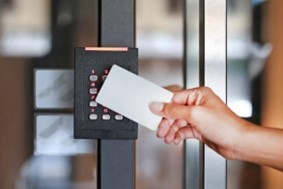
\includegraphics[width=\linewidth]{assets/rfid_access_control.jpg}
        \caption{\ac{rfid} Access Control Example}
        \label{fig:rfid-access-control}
    \end{minipage}
    \hfill
    \begin{minipage}{0.48\textwidth}
        \centering
        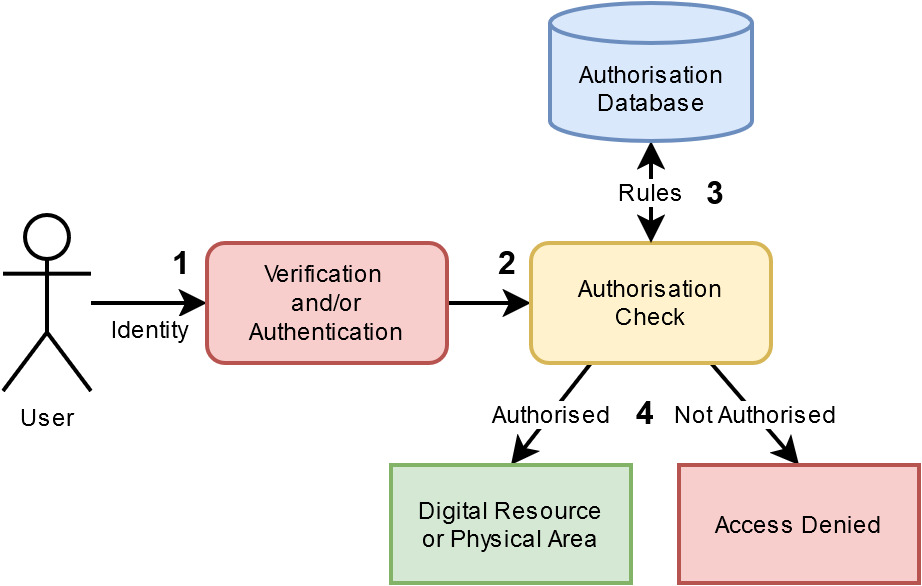
\includegraphics[width=\linewidth]{assets/access_control_flow.jpg}
        \caption{Access Control Flow Overview}
        \label{fig:access-control-flow}
    \end{minipage}
\end{figure}

The physical nature of \ac{rfid}-based controls means some vulnerabilities remain even after implementation of adequate encryption.
For instance, attackers are still able to steal the original key card.
Another traditional access control method, \ac{pin} codes, are also vulnerable to theft, despite being intangible.
Theft of \ac{pin} codes is even less perceptible due to there being no physical evidence \parencite{verkadaGuideSecurePhysical2024}.
These vulnerabilities remain predominantly due to a lack of authentication, allowing anyone to gain access to an area if in possession of valid credentials.

Trends in similar surveys suggest organisations are slowly moving away from traditional \ac{rfid}-based access control.
An alternative, but still token-based solution is smartphone authentication, which has seen a 7\% increase in use between 2022 and 2024 \parencite{ifsecglobal2022StatePhysical2022}.
Smartphone-based authentication does not suffer from the same vulnerabilities as traditional technologies, with the devices being harder to clone, or gain access to if stolen.
The sensors present in many modern phones (e.g., fingerprint scanners) and need for a \ac{pin}, enables \ac{mfa} --- enhancing security.

Usability of \ac{pacs} could also be improved.
As discussed, \ac{rfid}-based controls require users to carry a physical item holding their unique credentials.
In most if not all existing cases, users must direct their attention to or otherwise interact with the respective interface when providing credentials.
This could be considered inconvenient for users, especially those who are otherwise authorised and must stop to authenticate multiple times per day \parencite{ifsecglobalStatePhysicalAccess2024}

Although smartphone-based authentication reduces the total number of items a person must carry,
time penalties (although small) are still suffered, as users must stop to interact with their smartphone to authenticate.
There also remains a risk of theft, or of users misplacing their smartphone, making them unable to authenticate and undermining availability \parencite{maxsentiWhatPhysicalAccess2023}.

Many new access control solutions, some discussed in \ref{subsec:biometric-authentication-trends} below, enhance both security and usability by leveraging biometrics for authentication.
The nature of these systems and the type of data processed, however, has raised several ethical concerns regarding privacy, bias, and data misuse \parencite{prabhakarBiometricRecognitionSecurity2003,uwazuruikePoliceUseLive2025,parliamentaryofficeofscienceandtechnologyBiometricDataMisuse2024}.



\subsection{Biometric Authentication Trends in Physical Access Control}
\label{subsec:biometric-authentication-trends}

Biometric authentication methods assess unique biological characteristics --- inherence factors --- to determine identity.
The two main biometric characteristic categories are physiological: the physical parts of a person (e.g., fingerprints, face, or irises) and behavioural: the way a person interacts with an environment or system (e.g., walking style or keystroke pattern).

Figure \ref{fig:biometric-characteristics} below shows examples of (a) physiological and (b) behavioural characteristics.
Most \ac{pacs} that support biometric authentication leverage physiological factors \parencite{ifsecglobalStatePhysicalAccess2024}.
Behavioural factors, like gait --- explored as a viable alternative by this project --- could improve usability while maintaining the existing level of security we are used to \parencite{adminGaitRecognitionNext2024}.

\begin{figure}[H]
    \centering
    \begin{minipage}{0.48\textwidth}
        \centering
        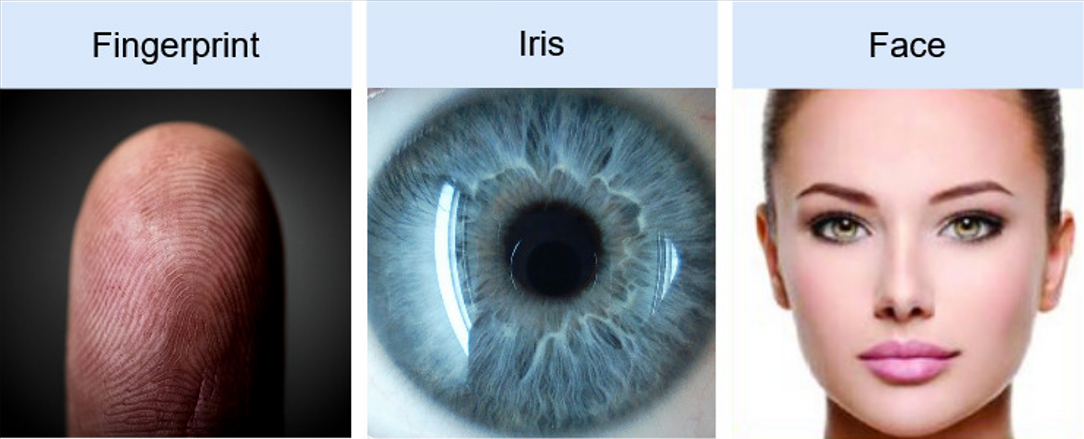
\includegraphics[width=\linewidth]{assets/physiological-characteristics.png}
        \subcaption{Physiological Characteristics}
        \label{fig:biometric-characteristics_a}
    \end{minipage}
    \hfill
    \begin{minipage}{0.48\textwidth}
        \centering
        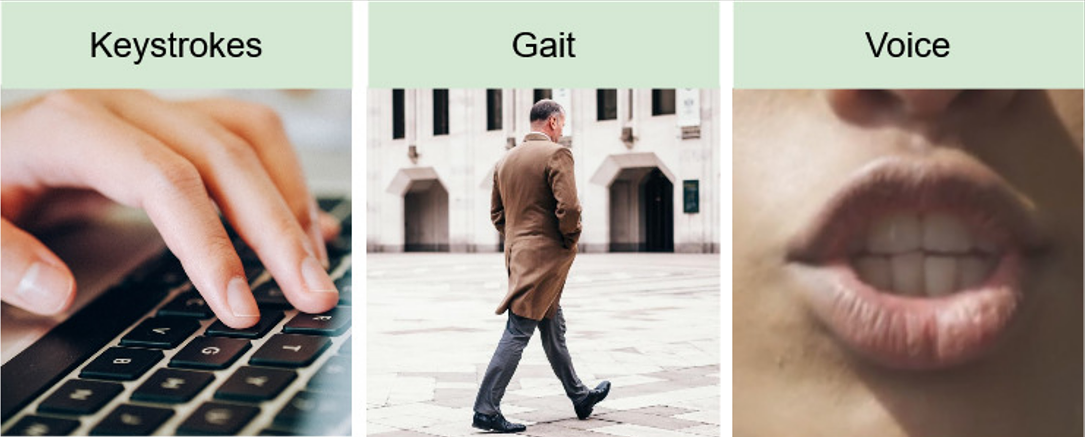
\includegraphics[width=\linewidth]{assets/behavioural-characteristics.png}
        \subcaption{Behavioural Characteristics}
        \label{fig:biometric-characteristics_b}
    \end{minipage}
    \caption{Examples of Biometric Characteristics}
    \label{fig:biometric-characteristics}
\end{figure}

In the context of \ac{pacs}, biometrics benefit usability by not requiring users to keep hold of a physical credential token, nor remember a secret value, with identities validated by assessing biological factors.
The reduced user burden also benefits security, as it is much harder for a person's likeness to be imitated convincingly enough to compromise the integrity of a biometric identification system \parencite{terranovasecurityEverythingYouNeed2023}.

\cite{ifsecglobalStatePhysicalAccess2024} also reported that 32\% of surveyed organisations made use of fingerprint, face, or iris-based biometric authentication.
Fingerprint recongition assesses the pattern or ridges on a persons fingertip(s).
A \cite{nationalinstituteofstandardsandtechnologyNISTStudyShows2004} study achieved a 98.6\% match accuracy using a single finger, rising to 99.9\% for for or more fingerprints.
Studies evaluating facial and iris recognition reported similar findings: 99.5\% and 98.6\% accuracy respectively \parencite{nationalinstituteofstandardsandtechnologyNISTEvaluatesFace2021,universityofbaghdadHighaccuracyModelsIris2024}

The type of information processed by biometric identification systems --- \ac{pii} --- raises concerns regarding privacy.
Although required to enable functionality, improper \ac{pii} handling can have a negative impact.
Stolen biometric records could be used for impersonation, or reveal confidential health information, for example \parencite{parliamentaryofficeofscienceandtechnologyBiometricDataMisuse2024}.
This risk necessitates secure and minimal \ac{pii} storage, where data handlers must only store what is needed, while it is needed.
Governments have published mandates for how \ac{pii} must be handled \parencite{informationcommissionersofficeBiometricDataGuidance2024}.

Additionally, the use of biometric identification systems by law enforcement, like the facial recognition technology installed as part of security upgrades in preparation for the London 2012 Olympics \parencite{homeofficeLondon2012Safe2011}, has led to ethical concerns regarding biases that could cause harm through misattribution or impact usability for minorities \parencite{uwazuruikePoliceUseLive2025,leslieUnderstandingBiasFacial2020}

Biometric recognition technologies use historic data to classify subsequent input based on similarities in features (e.g., to identify a person using an image of their face).
This requires the creation of datasets to train \ac{ml} models (see Section \ref{subsubsec:classification-techniques}) or to be used as a simpler reference database.
Failure to collect diverse sets of information --- many publically available datasets are unbalanced toward the default white male --- can result in embedded biases, impacting a system's effectiveness and the experience of minority users.
Facial recognition is one of the most common \ac{pacs} biometrics, yet has notoriously suffered.

\cite{leslieUnderstandingBiasFacial2020} reported that six out of a set of eight major facial recognition datasets studied contained more male images than female, and that 'six are composed of over eighty percent light-skinned faces'.
Biases like these can lead to misclassification, with darker-skinned women at times misclassified 'thirty-five times or more higher than for white men'.
In the context of access control, misclassification could undermine confidentiality, integrity, and availability by incorrectly identifying an unauthorised user as an authorised user, or vice versa.

Biases in surveillance and law enforcement systems can be more harmful.
Misclassification may lead to someone being incorrectly attributed to a crime they did not commit, for example \parencite{moyHowPoliceTechnology2019}.
The use of alternative biometric characteristics (i.e., gait) may help reduce these biases.
\ac{gr} is less affected by varying skin complexion, reducing the number of diversity dimensions to focus on when creating balanced datasets.
The most important dimensions for \ac{gr} appear to be sex and age, influencing body size and shape \parencite{guanGeneralizationPowerFace2014}.

Despite improving security and usability compared to traditional methods, the three most common biometric options do not significantly contribute to making authentication 'transparent'.
Fingerprint, iris, and most facial recognition systems require interaction with a physical interface before entry.
Of these, facial recognition is the most transparent, capable of operating from a distance in some implementations \parencite{boonedamFacialRecognitionSystem2024}.
Unfortunately, facial recognition often fails to work as expected in dynamic environments, with varying camera resolution, lighting conditions, and use of face coverings affecting data quality and impacting recognition accuracy \parencite{brajeIlluminationEffectsFace1998}.
These issues may be amplified when combined with concerns regarding biases in the datasets used to train the classification models (e.g., identifying darker-skinned individuals in low-light conditions).

Behavioural characteristics like gait (or keystroke analysis in a digital context) may enable less obtrusive authentication, eliminating several drawbacks of existing solutions, while maintaining an expected level of security.
These approaches work by assessing activity patterns over space and time to determine identity --- typically without requiring user's cooperation or even knowledge.
